\documentclass{standalone}
\usepackage[T1]{fontenc}
\usepackage[latin2]{inputenc}
\usepackage[english]{babel}
\usepackage{tikz}
\usetikzlibrary{calc,through,backgrounds,positioning,fit}
\usetikzlibrary{shapes,arrows,shadows}
 
\begin{document}
 
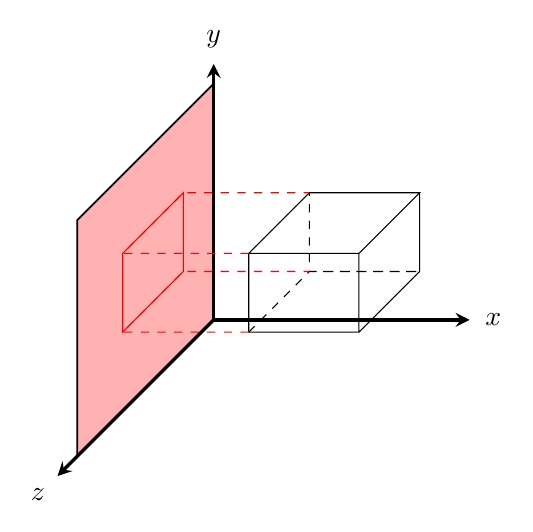
\begin{tikzpicture}[scale=1,inner sep=0.4mm]


\filldraw[fill=red!30!white,semithick] (0,0,0) -- (0,0,4.5)
 -- (0,3,4.5) -- (0,3,0) -- cycle;


\draw [->,>=stealth,very thick] (0,0,0) -- (3.25,0,0)
	node [right=4pt] {$x$};
\draw [->,>=stealth,very thick] (0,0,0) -- (0,3.25,0)
	node [above=4pt] {$y$};
\draw [->,>=stealth,very thick] (0,0,0) -- (0,0,5.15)
	node [below left=4pt] {$z$};
	
\draw  (3, 2, 1) -- (3, 1, 1) -- (3, 1, 3) -- (1.6, 1, 3) --
	   (3, 1, 3) -- (3, 2, 3) -- (1.6, 2, 3) -- (3, 2, 3) --
	   (3, 2, 1) -- (1.6, 2, 1) -- (1.6, 2, 3) -- (1.6, 1, 3);
	
\draw[dashed] (1.6, 1, 3) -- (1.6, 1, 1) -- (3, 1, 1) -- (1.6, 1, 1)
 -- (1.6, 2, 1);

\draw[dashed,draw=red] (1.6, 1, 3) -- (0,1,3) -- (0,1,1) -- (1.6, 1, 1);
\draw[dashed,draw=red] (1.6, 2, 3) -- (0,2,3) -- (0,2,1) -- (1.6, 2, 1);

\draw[draw=red] (0,1,3) -- (0,1,1) -- (0,2,1) -- (0,2,3) -- cycle;
	
\end{tikzpicture}
 
\end{document}